\section{About this template}
\label{sec:about}
% =============================================================================

The instructions below are suggestions to help your paper inherit a
consistent, Korea University-branded appearance. This template is a Korea University-styled adaptation of
the UC~Berkeley RAIL report class, which in turn derives from the Google DeepMind
technical-report template; it is distributed under the Creative Commons
Attribution--ShareAlike~4.0 license. This appendix collects the template instructions and examples. The manuscript entrypoint, \verb+main.tex+, contains a minimal paper skeleton.

The formatting behavior of the template is summarized in
Sections~\ref{sec:format}, \ref{sec:headings}, and \ref{sec:others} below.
Section~\ref{sec:extras} documents features specific to this Korea University template, and
Section~\ref{sec:building} explains how to compile the paper.

\subsection{What is in this template}
\label{sec:files}

This Overleaf-ready project separates the manuscript from reusable assets:
\begin{itemize}
  \item \verb+main.tex+ --- paper entrypoint and section inputs.
  \item \verb+kuarxiv.cls+ --- KU Crimson branding and layout.
  \item \verb+preamble.tex+ and \verb+command.tex+ --- packages and math macros.
  \item \verb+Sec/+ --- main paper sections, acknowledgments, and appendices.
  \item \verb+Sec/TemplateGuide.tex+ --- all template instructions and examples, including the sample table and author configurations.
  \item \verb+Figure/+ --- paper figures as standalone vector \verb+.pdf+ files.
  \item \verb+TemplateAssets/+ --- template-provided logo and PDF assets, separate from paper figures.
  \item \verb+Metadata/+ --- paper, author, affiliation, and abstract configuration.
  \item \verb+References/main.bib+ --- BibTeX references.
\end{itemize}

\subsection{The document class and its options}
\label{sec:options}

The paper begins with a single \verb+\documentclass+ line:
\begin{lstlisting}[style=promptstyle]
   \documentclass[11pt,letterpaper,logo]{kuarxiv}
\end{lstlisting}
The available options are:

\begin{itemize}
  \item \verb+10pt+ / \verb+11pt+ / \verb+12pt+ --- base font size.
  \item \verb+letterpaper+ --- US Letter paper (recommended for arXiv).
  \item \verb+twocolumn+ --- switch to a two-column layout (single column by
    default).
  \item \verb+logo+ --- show the KU logo at the bottom-right of the frontmatter card.
  \item \verb+nonumbering+ --- use unnumbered section headings.
  \item \verb+copyright+ --- add a copyright line to the first-page footer.
  \item \verb+internal+ --- mark the document as internal (enables the
    watermark/report-number footer).
  \item \verb+address+ --- print an affiliation line in the footer.
\end{itemize}

\subsection{Title, authors, and affiliations}
\label{sec:title}

Edit \verb+Metadata/paper.tex+ for the title, running title, and keywords;
\verb+Metadata/abstract.tex+ contains the abstract text. Author information is
configured in \verb+Metadata/authors.tex+. Each \verb+\KUAuthor+ entry takes
an author name, comma-separated affiliation numbers, and comma-separated role
keys. Supported roles are \texttt{equal}, \texttt{lead}, \texttt{corresponding},
and \texttt{senior}. Authors may have several affiliations and roles. Their
explanations appear once, automatically, below the author list. The author area contains affiliation details and email addresses without name prefixes. The official university logo sits beside the optional resource links below the abstract. The title and abstract share a light neutral rounded panel, followed
by the full contents before the first section. Complete metadata examples appear at the end of this guide.


\section{General formatting}
\label{sec:format}
% =============================================================================

The class fixes the page geometry, fonts, and spacing for you; you should not
need to touch any of it. The body text is set in Bitstream Charter
(\verb+XCharter+) with a matching Latin-Modern typewriter font, on US~Letter
paper. Paragraphs are separated by a half-line of vertical space and are not
indented, so a blank line in the source starts a visually distinct paragraph.

The title is set in Korea University Crimson, bold, and centered in the subtle neutral rounded frontmatter panel. All headings are bold and flush left. Follow the guidance in Section~\ref{sec:others} regarding citations,
figures, tables, and mathematics, and keep the margins, text width,
and font sizes defined in the class file.


% =============================================================================


\section{Headings}
\label{sec:headings}
% =============================================================================

First-level headings are bold and, by default, numbered. Use \verb+\section+,
\verb+\subsection+, and \verb+\subsubsection+ for the first three levels. If you
prefer unnumbered headings throughout, pass the \verb+nonumbering+ class option.

\subsection{Second-level headings}
\label{sec:second}

Second-level headings are produced with \verb+\subsection+ and are slightly
smaller than first-level headings.

\subsubsection{Third-level headings}
\label{sec:third}

Third-level headings are produced with \verb+\subsubsection+ and are set in bold
italic.

\paragraph{Paragraph headings.}
There is also a \verb+\paragraph+ command, which sets its heading in bold, flush
left, and run into the start of the paragraph, as shown here. Use it for the
finest level of structure.


% =============================================================================


\section{Citations, figures, tables, and mathematics}
\label{sec:others}
% =============================================================================

These instructions apply to every paper written with the template.

\subsection{Citations within the text}
\label{sec:citations}

The \verb+natbib+ package is loaded in \verb+preamble.tex+ and configured for a
numeric, square-bracket citation style via \verb+\setcitestyle{numbers,square}+; the
bibliography style is \verb+IEEEtranN+. Use \verb+\citet+ for a textual citation
that reads as part of the sentence, and \verb+\citep+ for a parenthetical one.
For example, \verb+\citet{Alpher02}+ produces ``\citet{Alpher02} showed that
frobnication is possible,'' whereas \verb+\citep{Alpher03,Alpher04}+ produces a
grouped parenthetical citation \citep{Alpher03,Alpher04}. Supplementary material
can be cited in the same way \citep{Authors14}. Any consistent citation style is
acceptable; to change it, edit the \verb+\setcitestyle+ line in the preamble and
the \verb+\bibliographystyle+ line in \verb+main.tex+.

\subsection{Footnotes}
\label{sec:footnotes}

Use footnotes sparingly. Indicate a footnote with the \verb+\footnote+
command,\footnote{This is a sample footnote; it is typeset at the bottom of the
page on which it appears.} and note that footnote marks are placed \emph{after}
punctuation.

\subsection{Figures}
\label{sec:figures}

All artwork should be neat, clean, and legible, and figures are numbered
consecutively. The figure caption is placed \emph{below} the figure. Include
raster or vector art with \verb+\includegraphics+ from the \verb+graphicx+
package (loaded for you), and it is best to give the width as a multiple of
\verb+\linewidth+ so the figure scales with the text block:
\begin{lstlisting}[style=promptstyle]
   \includegraphics[width=0.8\linewidth]{Figure/your_figure.pdf}
\end{lstlisting}
Figure~\ref{fig:sample} loads a sample vector PDF from \verb+Figure/+.
You may use color, but try to keep captions and the paper body legible in both
color and grayscale.

\begin{figure}[t]
  \centering
  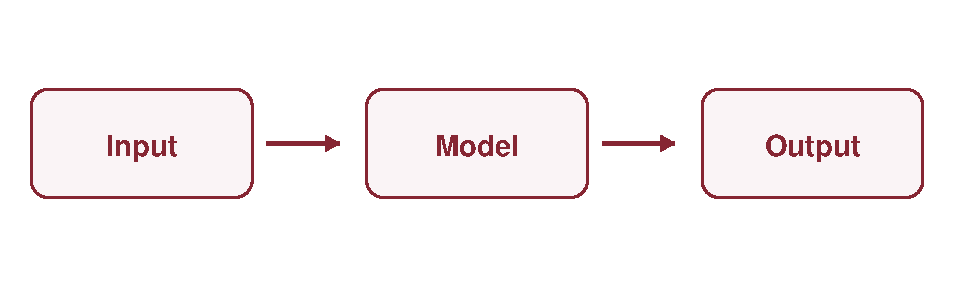
\includegraphics[width=0.85\linewidth]{Figure/example_pipeline.pdf}
  \caption{A simple illustrative pipeline stored as a separate vector PDF.}
  \label{fig:sample}
\end{figure}

\subsection{Tables}
\label{sec:tables}

All tables should be centered, and the caption is placed \emph{above} the table.
Publication-quality tables typically avoid vertical rules; the \verb+booktabs+ package
(loaded for you) provides \verb+\toprule+, \verb+\midrule+, and \verb+\bottomrule+
for clean horizontal rules, as illustrated in Table~\ref{tab:sample}.

% Original table source, consolidated into the template guide.
\begin{table}[t]
  \caption{Sample table caption. Explain what the table shows and add a key
  take-away message to the caption.}
  \label{tab:sample}
  \centering
  \begin{tabular}{lll}
    \toprule
    \multicolumn{2}{c}{Part} \\
    \cmidrule(r){1-2}
    Name     & Description     & Size ($\mu$m) \\
    \midrule
    Dendrite & Input terminal  & $\approx$100  \\
    Axon     & Output terminal & $\approx$10   \\
    Soma     & Cell body       & up to $10^6$  \\
    \bottomrule
  \end{tabular}
\end{table}


\subsection{Mathematics, theorems, and definitions}
\label{sec:math}

Use \LaTeX{} (or \verb+amsmath+) commands for display math; avoid bare
\verb+$$...$$+. Numbered equations use the \verb+equation+ environment:
\begin{equation}
  \label{eq:sample}
  \mathcal{L}(\theta)
  = \frac{1}{n}\sum_{i=1}^{n} \ell\!\big(f_\theta(x_i), y_i\big).
\end{equation}
The macros in \verb+command.tex+ provide common shortcuts (for example
\verb+\R+ for $\R$, \verb+\E+ for $\E$, and \verb+\argmin+ / \verb+\argmax+).

The file \verb+command.tex+ also defines a family of theorem-like environments
that share a single counter: \verb+definition+, \verb+theorem+, \verb+lemma+,
\verb+corollary+, \verb+proposition+, \verb+remark+, \verb+observation+,
\verb+claim+, \verb+example+, \verb+assumption+, and \verb+conjecture+.
For instance:

\begin{definition}[Frobnication]
\label{def:frob}
A map $f:\mathcal{X}\to\mathcal{Y}$ is \emph{frobnicable} if there exists a foo
filter $g$ such that $g\circ f$ is the identity on $\mathcal{X}$.
\end{definition}

\begin{theorem}
\label{thm:frob}
Every frobnicable map is injective.
\end{theorem}

\begin{proof}
If $f(x)=f(y)$, applying the left inverse $g$ from Definition~\ref{def:frob} gives $x=y$; the \verb+proof+ environment supplied by \verb+amsthm+ adds the closing
\emph{QED} symbol automatically.
\end{proof}


% =============================================================================


\section{Extra features of the Korea University template}
\label{sec:extras}
% =============================================================================

The following features go beyond a plain article class and are specific to this
template.

\subsection{Header and footer}
\label{sec:headerfooter}

On the first page, the \verb+logo+ option prints the Korea University logo beside the optional resource links below the abstract and, if you set \verb+\paperurl={...}+, its value is printed as a link in
the top-right corner. From the second page onward, the header shows the
\verb+\runningtitle+ centered and the page number in the bottom-right. The
\verb+copyright+, \verb+internal+, and \verb+address+ options add the
corresponding lines to the footer.

\subsection{Corresponding author, paper URL, and keywords}
\label{sec:metadata}

Several optional metadata commands are available:
\begin{itemize}
  \item \verb+\keywords{a, b, c}+ --- prints a keyword list beneath the abstract
    within the neutral frontmatter panel (as shown on the first page).
  \item \verb+\paperurl={...}+ --- prints a project or preprint URL in the
    first-page header.
  \item \verb+\correspondingauthor={...}+ --- enables a corresponding-author note
    in the first-page footer.
  \item \verb+\reportnumber={...}+ --- prints a report number in the footer when
    the \verb+internal+ option is active.
\end{itemize}

\subsection{Callout boxes}
\label{sec:callout}

The template preloads \verb+tcolorbox+. The preamble defines a \verb+simpleElegantQuote+
environment for highlighting a key sentence:

\begin{simpleElegantQuote}
A paper template should get out of your way: set the type once, set it well, and
let the author think about the ideas rather than the margins.
\end{simpleElegantQuote}

\subsection{Code and prompt listings}
\label{sec:listings}

\verb+preamble.tex+ defines a \verb+promptstyle+ for the \verb+listings+ package,
useful for verbatim code, configuration, or LLM prompts:

\begin{lstlisting}[style=promptstyle]
System: You are a helpful assistant.
User: Summarize the Korea University arXiv template in one sentence.
Assistant: It is a Korea University-branded article class that fixes fonts, colors, and
           layout so you only have to write the paper.
\end{lstlisting}


% =============================================================================


\section{Building the paper}
\label{sec:building}
% =============================================================================

Prepare submission files with paper size ``US~Letter'' and generate the PDF
directly with \verb+pdflatex+ so that only Type~1 or embedded TrueType fonts are
used. The simplest way is \verb+latexmk+, which runs the full
\verb+pdflatex+\,$\rightarrow$\,\verb+bibtex+\,$\rightarrow$\,\verb+pdflatex+ cycle
so that citations and cross-references resolve in one command:
\begin{lstlisting}[style=promptstyle]
   latexmk -pdf -interaction=nonstopmode main.tex
\end{lstlisting}
This produces \verb+main.pdf+. To remove build artifacts, run
\verb+latexmk -c+ (keep the PDF) or \verb+latexmk -C+ (also remove the PDF). See
\verb+README.md+ for environment-specific notes.


% =============================================================================


\section*{Acknowledgments}
\phantomsection\addcontentsline{toc}{section}{Acknowledgments}
% =============================================================================

Use an unnumbered first-level heading for acknowledgments, placed at the end of
the paper before the references. This Korea University template adapts the UC~Berkeley RAIL
report class and the Google DeepMind technical-report template, used under the
CC~BY-SA~4.0 license.


\section{Additional material}
\label{app:extra}
% =============================================================================

Content placed after \verb+\appendix+ is lettered rather than numbered
(Appendix~\ref{app:extra}), and the axiom-style counters defined in
\verb+command.tex+ reset so they read \textit{G.1}, \textit{G.2}, and so on. Use
the appendix for proofs, extended tables, additional experiments, or verbatim
prompts that support --- but are not essential to --- the main text.

\subsection{Theorem environment gallery}
These statements and the sample bibliography entries are fictional typesetting examples.
\begin{lemma}An illustrative \texttt{lemma} environment.\end{lemma}
\begin{remark}An illustrative \texttt{remark} environment.\end{remark}
\begin{corollary}An illustrative \texttt{corollary} environment.\end{corollary}
\begin{proposition}An illustrative \texttt{proposition} environment.\end{proposition}
\begin{observation}An illustrative \texttt{observation} environment.\end{observation}
\begin{claim}An illustrative \texttt{claim} environment.\end{claim}
\begin{example}An illustrative \texttt{example} environment.\end{example}
\begin{assumption}An illustrative \texttt{assumption} environment.\end{assumption}
\begin{axiom}An illustrative \texttt{axiom} environment.\end{axiom}
\begin{property}An illustrative \texttt{property} environment.\end{property}
\begin{conjecture}An illustrative \texttt{conjecture} environment.\end{conjecture}

\subsection{Additional math shortcuts}
\[X\independent Y,\qquad\Tr{A},\qquad\Wass(P,Q),\qquad\EE[X].\]

\section{Author and resource configuration examples}
\label{app:metadataexamples}
Copy a complete author example into \verb+Metadata/authors.tex+. All identities below are illustrative. The role keys and multi-affiliation interface are unchanged.

\Needspace{8\baselineskip}
\subsection{Single}
\begin{lstlisting}[style=promptstyle]
% Illustrative metadata; replace all placeholder identities.
\KUResetAuthors
\KUAuthor{Author Name}{1}{corresponding}
\KUAffiliation{1}{Department of Artificial Intelligence, Korea University, Seoul, Republic of Korea}
\KUEmail{Author Name}{author@korea.ac.kr}
\end{lstlisting}

\Needspace{8\baselineskip}
\subsection{Multi same}
\begin{lstlisting}[style=promptstyle]
% Illustrative metadata; replace all placeholder identities.
\KUResetAuthors
\KUAuthor{Minji Kim}{1}{equal}
\KUAuthor{Jisoo Park}{1}{equal}
\KUAuthor{Alex Lee}{1}{corresponding}
\KUAffiliation{1}{Department of Artificial Intelligence, Korea University, Seoul, Republic of Korea}
\KUEmail{Alex Lee}{alex.lee@korea.ac.kr}
\end{lstlisting}

\Needspace{8\baselineskip}
\subsection{Multi affiliations}
\begin{lstlisting}[style=promptstyle]
% Illustrative metadata; replace all placeholder identities.
\KUResetAuthors
\KUAuthor{Minji Kim}{1,2}{equal}
\KUAuthor{Jisoo Park}{2}{equal}
\KUAuthor{Alex Lee}{1}{corresponding}
\KUAffiliation{1}{Department of Artificial Intelligence, Korea University, Seoul, Republic of Korea}
\KUAffiliation{2}{Example Research Institute, Seoul, Republic of Korea}
\KUEmail{Alex Lee}{alex.lee@korea.ac.kr}
\end{lstlisting}

\Needspace{8\baselineskip}
\subsection{Combined}
\begin{lstlisting}[style=promptstyle]
% Illustrative metadata; replace all placeholder identities.
\KUResetAuthors
\KUAuthor{Minji Kim}{1,2}{equal,lead,corresponding}
\KUAuthor{Jisoo Park}{2}{equal}
\KUAuthor{Alex Lee}{1}{senior,corresponding}
\KUAuthor{Sam Choi}{1,2}{senior}
\KUAffiliation{1}{Department of Artificial Intelligence, Korea University, Seoul, Republic of Korea}
\KUAffiliation{2}{Example Research Institute, Seoul, Republic of Korea}
\KUEmail{Minji Kim}{minji.kim@korea.ac.kr}
\KUEmail{Alex Lee}{alex.lee@korea.ac.kr}
\end{lstlisting}

\Needspace{8\baselineskip}
\subsection{Long}
\begin{lstlisting}[style=promptstyle]
% Illustrative metadata; replace all placeholder identities.
\KUResetAuthors
\KUAuthor{Example Author 1}{1}{corresponding}
\KUAuthor{Example Author 2}{2}{}
\KUAuthor{Example Author 3}{3}{}
\KUAuthor{Example Author 4}{1}{}
\KUAuthor{Example Author 5}{2}{}
\KUAuthor{Example Author 6}{3}{}
\KUAuthor{Example Author 7}{1}{}
\KUAuthor{Example Author 8}{2}{}
\KUAuthor{Example Author 9}{3}{}
\KUAuthor{Example Author 10}{1}{}
\KUAuthor{Example Author 11}{2}{}
\KUAuthor{Example Author 12}{3}{}
\KUAuthor{Example Author 13}{1}{}
\KUAuthor{Example Author 14}{2}{}
\KUAuthor{Example Author 15}{3}{}
\KUAuthor{Example Author 16}{1}{}
\KUAuthor{Example Author 17}{2}{}
\KUAuthor{Example Author 18}{3}{}
\KUAuthor{Example Author 19}{1}{}
\KUAuthor{Example Author 20}{2}{}
\KUAuthor{Example Author 21}{3}{}
\KUAuthor{Example Author 22}{1}{}
\KUAuthor{Example Author 23}{2}{}
\KUAuthor{Example Author 24}{3}{}
\KUAffiliation{1}{Department of Artificial Intelligence, Korea University, Seoul, Republic of Korea}
\KUAffiliation{2}{Example Research Institute, Seoul, Republic of Korea}
\KUAffiliation{3}{Example Collaborative Research Center, Seoul, Republic of Korea}
\KUEmail{Example Author 1}{example.author@korea.ac.kr}
\end{lstlisting}

\subsection{Optional resource links}
Replace these placeholders or clear the list to omit it:
\begin{lstlisting}[style=promptstyle]
\KUResetResources
\KUResource{Code}{https://example.org/code}
\KUResource{Homepage}{https://example.org/project}
\KUResource{Dataset}{https://example.org/dataset}
\end{lstlisting}
\subsection{Contribution labels}
Role notes are printed once, in the order equal, lead, corresponding, senior.
Use the following command to customize a label:
\begin{lstlisting}[style=promptstyle]
\KUContribution{lead}{Project coordination}
\end{lstlisting}

\Needspace{20\baselineskip}
\subsection{Original frontmatter examples}
The original title, keywords, resources, and instructional abstract are retained below as source examples. For a new paper, edit the three active files in \verb+Metadata/+; the standalone sample table is now consolidated in this guide.
\begin{lstlisting}[style=promptstyle]
% Research Plan, Technical Report, or arXiv Paper: edit these values only.
\title{The Korea University Academic Template:\\Research Plans, Technical Reports, and arXiv Papers}
\runningtitle{Research Plans}
\keywords{Korea University, \LaTeX{}, academic writing, reproducible research}

% Illustrative placeholders only: replace with your real project links, or remove.
\KUResetResources
\KUResource{Code}{https://example.org/code}
\KUResource{Homepage}{https://example.org/project}
\KUResource{Dataset}{https://example.org/dataset}
\end{lstlisting}
\begin{quote}
This document is a working example and usage guide for a reusable Korea University-styled academic template. It uses a very light rounded frontmatter panel, Crimson accents, compact author metadata, and a shared resource--university information block. Manuscript sections and appendices live in \texttt{Sec/}, table sources in \texttt{Table/}, vector figures in \texttt{Figure/}, and template resources in \texttt{TemplateAssets/}. Paper and author information are configured in \texttt{Metadata/}. Replace these examples with your own research plan, technical report, or paper while preserving the directory conventions.
\end{quote}

\subsection{Automatic author records}
Use the three-field interface for new documents. Shared units are numbered automatically, and emails are displayed without names or colons:
\begin{lstlisting}[style=promptstyle]
\KUResetAuthors
\KUAddAuthor{Alice Kim}{Department, University A}{alice@example.org}
\KUAddAuthor{Bob Lee}{Department, University A}{bob@example.org}
\KUAddAuthorMulti[corresponding]{Carol Park}
  {{Department, University A},{School, University B}}
  {carol@example.org}
\end{lstlisting}
Each complete unit in a multi-unit list must have its own braces. The manual author and affiliation commands in the preceding examples remain supported. Repeated units and email addresses are rendered once; author entries remain distinct.
